\documentclass[border=4pt]{standalone}
\usepackage{fontspec}
\usepackage{amsmath}
\usepackage{unicode-math}
\setmainfont{Latin Modern Roman}
\setmathfont{Latin Modern Math}
\usepackage{pgfplots}
\usepackage{pgfplotstable}
\pgfplotsset{compat=1.18}
\usepackage{tkz-euclide}
\usetikzlibrary{arrows.meta,calc,angles,quotes,patterns,3d,backgrounds}
\definecolor{ink}{HTML}{123428}
\definecolor{asy}{HTML}{475569}
\definecolor{mint}{HTML}{86e0bd}
\tikzset{asym/.style={asy, line width=0.9pt, dash pattern=on 5pt off 3.5pt},
         guide/.style={gray!70, line width=0.6pt, densely dotted},
         dot/.style={circle, inner sep=0pt, minimum size=5pt, draw=white, line width=0.5pt},
         odot/.style={circle, inner sep=0pt, minimum size=5.5pt, fill=white, line width=1pt},
         lab/.style={font=\footnotesize, inner sep=1.5pt, text=ink}}
\begin{document}
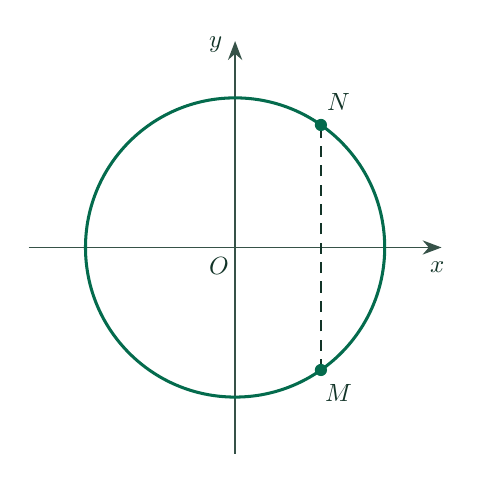
\begin{tikzpicture}
\draw[ink!85, line width=0.7pt, -{Stealth[length=2.4mm]}] (-2.622,0.000) -- (2.622,0.000);
\draw[ink!85, line width=0.7pt, -{Stealth[length=2.4mm]}] (0.000,-2.622) -- (0.000,2.622);
\draw[color={rgb,255:red,4;green,107;blue,77}, line width=1.1pt] (0,0) circle (1.900);
\draw[ink, line width=0.7pt, dash pattern=on 4pt off 3pt] (1.090,-1.556) -- (1.090,1.556);
\node[font=\small, text=ink] at (2.572,-0.25) {$x$};
\node[font=\small, text=ink] at (-0.25,2.572) {$y$};
\fill[color={rgb,255:red,4;green,107;blue,77}] (1.090,-1.556) circle (2.2pt);
\fill[color={rgb,255:red,4;green,107;blue,77}] (1.090,1.556) circle (2.2pt);
\node[font=\small, text=ink, inner sep=0.5pt] at (1.296,-1.851) {$M$};
\node[font=\small, text=ink, inner sep=0.5pt] at (1.296,1.851) {$N$};
\node[font=\small, text=ink, inner sep=0.5pt] at (-0.200,-0.240) {$O$};
\end{tikzpicture}
\end{document}
